\begin{tcolorbox}[colback=blue!5!white, %
  colframe=blue!75!black, %
  title=\textbf{Predictor-Corrector Path-following for RT-OC and NMPC}]
  $p=x_0$ is the parameter on which parameter optimization hinges.
  ``Generalized tangential predictor'' can jump over active set changes (that's
  where the trajectory manifold has kinks).
  \begin{itemize}
  \item \textbf{GMRES method of Ohtsuka}
    \begin{itemize}
    \item Sequential (single-shooting)
    \item IP method, with fixed $\tau>0$
    \item Exact Hessian\\
    \end{itemize}
    \includegraphics[width=0.8\textwidth]{ohtsuka}
  \item \textbf{Advanced step controller}
    \begin{itemize}
    \item Solve NLP for a predicted parameter $\bar{p}_{k+1}$
    \item get $\nabla_p w^*(p)$ from KKT matrix
    \item when real parameter $p_{k+1}$ arrives:
      \begin{align*}
        y^*_{k+1} = \bar{y}_{k+1}(\bar{p}_{k+1})+\nabla_pw^*(\bar{p}_{k+1})(p_{k+1} - \bar{p}_{k+1})
      \end{align*}
    \end{itemize}
    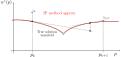
\includegraphics[width=0.8\textwidth]{advanced_step}
  \item \textbf{Real-Time Iteration Scheme}
    \begin{itemize}
    \item Preprocess SQP with inputs $y_k, p_{k+1}$:
      \begin{align*}
        \min_w \quad&f(w) \\ \mathrm{s.t.}\quad& g(w) + M\cdot p = 0,& M:=[\mathbb{I}^{n_x}, 0, \dots] \\ & h(w) \le 0
      \end{align*}
      \begin{align*}
        \Rightarrow \min_w \quad & \nabla_w f(w)^T\cdot (w-w_k) + 0.5 \nabla^2_w \mathcal{L}(y)\cdot(w-w_k) \\
        \mathrm{s.t.}\quad& g(w) + \nabla_w g(w_k)\cdot(w-w_k) - Mp_{k+1} = 0 \\
        & h(w) + \nabla_w h(w_k)\cdot(w-w_k)\le 0
      \end{align*}
    \item Just perform \emph{one} linearization and one QP solution
    \item Often used: Gauss-Newton-Hessian
    \item Works well when the active set changes faster than the linearized
      system matrices
    \item Warm-start the state
    \end{itemize}

  \end{itemize}
\end{tcolorbox}

%%% Local Variables:
%%% coding: utf-8
%%% mode: latex
%%% TeX-engine: xetex
%%% TeX-master: "../HelpSheet"
%%% End: